\section{Définition des Boucles Optiques}

\paragraph{} Afin de déployer une nouvelle infrastructure réseau acceptant la ToIP dans le but de remplacer à terme l'ensemble des téléphones analogiques par des téléphones numériques (y compris les téléphones des secours), il est nécessaire de pouvoir assurer le transfert de données en toute circonstances. La sécurité du réseau doit être assurée par une double connexion de chaque bâtiment au réseau optique du campus. De cette manière, même en cas de défaillance d'une fibre, les données pourront toujours circuler. L'unique boucle optique actuellement disponible sur le campus ne répond pas aux exigences de sécurité citées ci-dessus. Elle est également déployée dans des fourreaux anciens et ne répondant pas aux normes de sécurité actuelles. Enfin, les fibres sont principalement des fibres optiques multimode ne permettant pas un débit suffisant pour gérer à la fois le réseau de données et le réseau téléphonique qui devront passer par les mêmes voies.

\paragraph{} De grands travaux d'aménagement seront effectués lors de la mise en place du projet de déploiement de ToIP sur le campus. Deux nouvelles connexions de fibres optiques seront mises en place : une boucle et une étoile. Ces connexion seront installées dans de nouveaux fourreaux enterrés dans tout le campus. Nous utiliserons des fibres monomodes, les nouvelles connexions formeront un réseau permettant à chaque bâtiment d'avoir deux accès indépendants au réseau global du campus. Les figures ci-dessous présentent les deux connexions avec les nœuds optiques associés.

\paragraph{} Les boucles seront créées selon un schéma de déploiement en étoile autour du bâtiment Jacquard qui représente le cœur du réseau. La boucle (qui est la connexion principale) est en plus conçue pour transporter les données d'un nœud à l'autre même en cas de section d'une partie de la boucle.


\begin{figure}[h]
  \caption{\label{Plan_boucle1} Première boucle optique}
  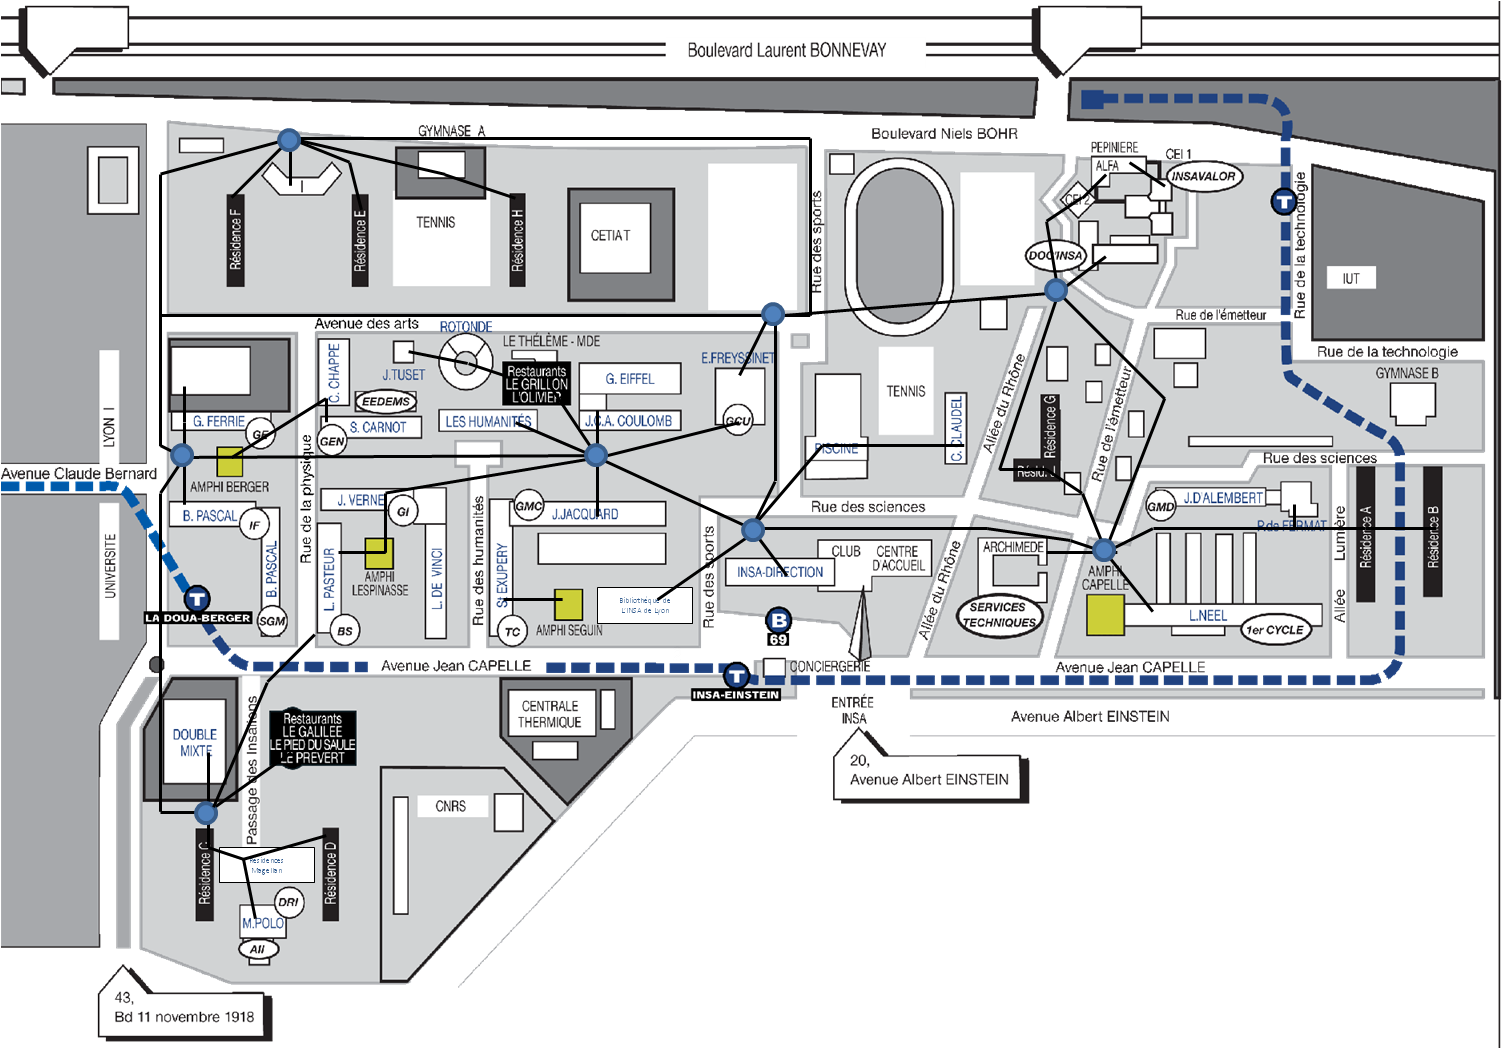
\includegraphics[scale=0.6]{Boucle1.png}
\end{figure}

\begin{figure}[h]
  \caption{\label{Plan_boucle2} Deuxième boucle optique}
  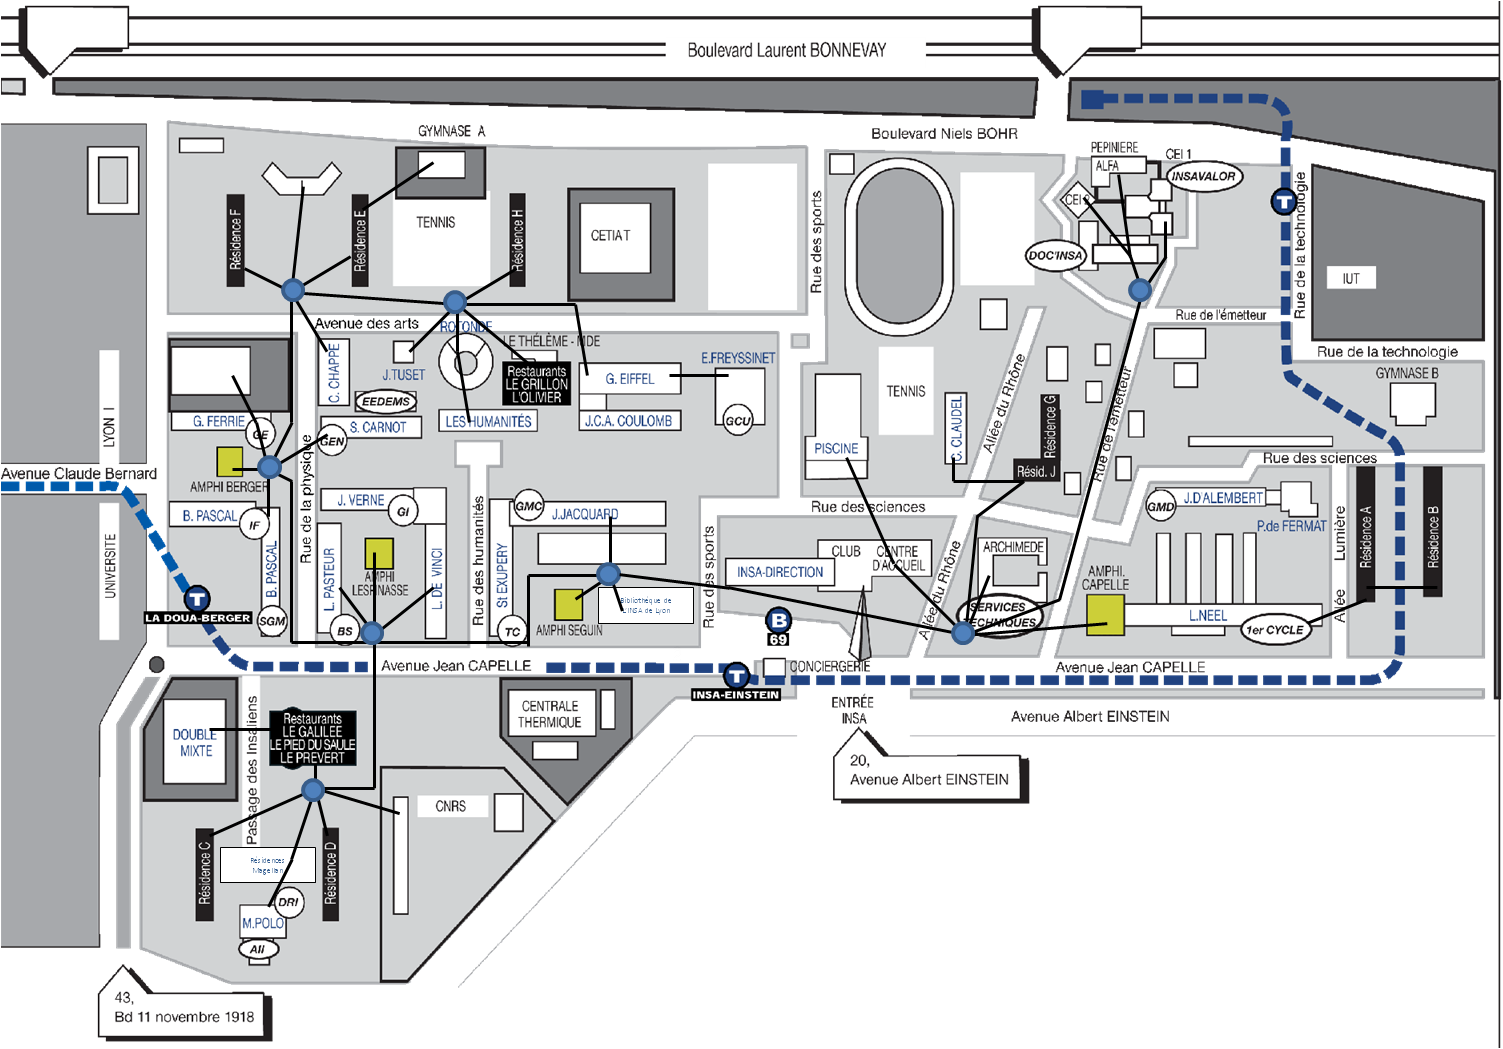
\includegraphics[scale=0.6]{Boucle2.png}
\end{figure}
~\\

\paragraph{} Nous pouvons remarquer que le déploiement de ces boucles conduira à la construction de 16 nœuds optiques et entrainera la pose de 6000 mètres de fourreaux pour la boucle 1 et 4500 mètres pour la seconde. Ces nœuds seront les points de convergence des fourreaux. L'alimentation électrique de ces nœuds se fera par câbles électriques enterrés dans des fourreaux parallèles aux fourreaux de fibre optique. Cette connexion permettra non seulement de n'avoir à effectuer qu'une seule tranchée pour les fibres et l'alimentation mais également de permettre de centraliser l'alimentation des différents nœuds et locaux techniques au bâtiment Jacquard ce qui permettra d'y installer les équipements de protection en cas de coupure de courant sur le campus (onduleur sur batterie, groupe électrogène).

\paragraph{} Deux chambres de tirage de fibre optique seront créées par bâtiment raccordé au boucles (une par connexion). Ces deux chambres de tirage raccorderont chaque bâtiment par deux emplacements distincts et espacés géographiquement afin de réduire les risques de déconnexion des bâtiments en cas de sinistre dans une partie de celui-ci.

\paragraph{} Comme présenté dans les plans, les fourreaux seront placés entre les bâtiments connectés. Afin de limiter le nombre de nœuds optiques, certaines fibres passeront à l'intérieur d'un bâtiment et seront redirigées vers un autre fourreau de sortie dans le local technique de ce dernier pour connecter un bâtiment voisin. Afin de prévenir de tout risque causé par le destruction de fourreaux aux abords des locaux techniques, chaque bâtiment connecté au réseau disposera de deux points d'entrées bien distincts pour les connexions des deux boucles optiques (en général : un point d'entrée pour la première boucle au niveau du local technique, une deuxième point d'entrée pour la seconde à l'autre bout du bâtiment. La fibre sera amenées au local par le câblage interne du bâtiment).

\paragraph{} La plupart des bâtiments du campus sont déjà équipés de locaux techniques pour la gestion de leur parc informatique. Lors de la mise en place des fourreaux pour la connexion d'un bâtiment, ces locaux techniques seront rénovés et équipés avec le matériel nécessaire à la gestion des deux nouvelles connexions. La rénovation passera par le changement des switchs qui seront utilisés par les téléphones en switchs POE, l'installation de climatisation dans les locaux (les switchs POE émettent plus de chaleur en fonctionnement que les switchs normaux), la création des deux nouvelles chambres de tirage décrites ci-dessus.

\paragraph{} Si la place disponible dans les locaux techniques d'un bâtiment n'est pas suffisante, de nouveaux locaux pourront être créés après destruction des anciens. La politique sera alors la création d'un ou deux locaux techniques par bâtiment (en fonction de la taille de ce dernier). Ce locaux techniques seront situés le plus possible aux étages médians des bâtiments afin de limiter la longueur des câbles Ethernet dans les bâtiments. 